\section{MOS Stromspiegel}

\begin{minipage}[t]{0.48\columnwidth}
    Stromspiegel werden in \textbf{jeder} analogen integrierten Schaltung eingesetzt.
    Die möglichen Anwendungen sind:
\end{minipage}
\hfill
\begin{minipage}[t]{0.48\columnwidth}
    \begin{itemize}
        \item um Arbeitspunkte einzustellen
        \item als Eingangsstufen von OpAmps
        \item als grosse Lastwiderstände in Verstärkerschaltungen
    \end{itemize}
\end{minipage}


\subsection{Einfache Stromspiegel (3 Pol)}

\begin{minipage}[c]{0.35\columnwidth}
    \raggedright
    \begin{outline}
        \1 Drei Anschlüsse: \\
            SUPPLY, IN, OUT
        \1 Eingangstransistor als \textbf{Diode} beschaltet
        \1 \textbf{Ausgangstransistor muss in Sättigung bleiben}
        \1 $V_{\rm GS,1} = V_{\rm GS,2}$
    \end{outline}
\end{minipage}
\hfill
\begin{minipage}[c]{0.64\columnwidth}
    \begin{tabular}{c c@{}}
        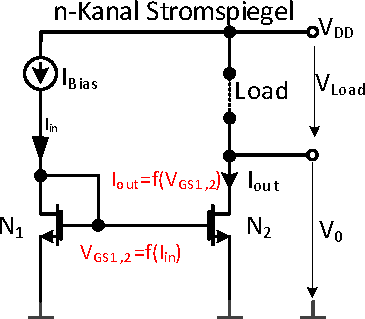
\includegraphics[height=2.3cm]{images/06_stormspiegel_nKanal.pdf} & 
        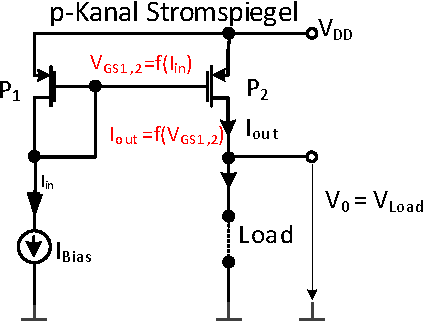
\includegraphics[height=2.3cm]{images/06_stormspiegel_pKanal.pdf}
    \end{tabular}
\end{minipage}


\paragraph{Wichtige Parameter}  % CHECK [Simi]: Ich weiss nicht so recht wo hin mit diesem Zeug...

\begin{minipage}[t]{0.48\columnwidth}
    \begin{outline}
        \1 Ausgangsstom $I_\text{out}$ berechnet sich aus Stromspiegelverhältnis $k$
    \end{outline}
\end{minipage}
\hfill
\begin{minipage}[t]{0.48\columnwidth}
    \begin{outline}
        \1 Eingangsimpedanz (real): $r_i = \qty{0}{\ohm}$
        \1 Ausgangsimpedanz (real): $r_o = \infty \, \qty{}{\ohm}$
    \end{outline}
\end{minipage}



\subsubsection{Arbeitspunkt festlegen}

\paragraph{Eingangsseite}

Referenzstrom aus Stromquelle oder Einstellung über Widerstand $R$

\vspace{-0.2cm}

\[
    I_\text{in} = I_\text{ref} \qquad \text{oder} \qquad I_\text{in} = \frac{V_{DD} - V_{\rm in}}{R}
\]

wobei sich die Eingangsspannung $V_{\rm in} = V_{\rm GS,1}$ aus dem Eingangsstrom berechnet als

\vspace{-0.2cm}

\[
    V_\text{in} = V_{\rm GS,1} = V_{\text{T, N}_1} + \sqrt{\frac{2 I_\text{in}}{\mu C_\text{ox}\frac{W_{\rm in}}{L_{\rm in}}}}
\]



\paragraph{Ausgangsseite}

Für Eingangs- und Ausgangstransistor soll unbedingt \textbf{das gleiche $\bm{L}$} verwendet werden.
Bei verschiedenen $L$ muss die \cbl{Kanallängenmodulation} berücksichtigt werden!

\vspace{-0.2cm}

\[
    k = \frac{I_\text{out}}{I_\text{in}} = \frac{W_\text{out}/L_\text{out}}{W_\text{in}/L_\text{in}} \cbl{ \cdot \frac{1 + \lambda_{\rm out} \cdot V_{\rm DS,out}}{1 + \lambda_{\rm in} \cdot V_{\rm DS,in}} }   \qquad \quad
    V_\text{out} \geq V_\text{DS, sat $\text{N}_2$} = \sqrt{\frac{2 I_\text{out}}{\mu C_\text{ox}\frac{W_{\rm out}}{L_{\rm out}}}}
\]


\begin{minipage}[t]{0.48\columnwidth}
    \subsubsection{Kleinsignalersatzschaltung}

    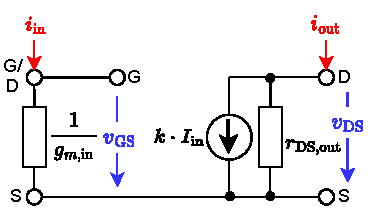
\includegraphics[width=\columnwidth, align=t]{images/06_stromspiegel_kleinsignalersatzschaltung.pdf}
\end{minipage}
\hfill
\begin{minipage}[t]{0.48\columnwidth}
    \raggedright
    \subsubsection{Anwendungen}

    \begin{outline}
        \1 Senken-Quellen-Inversion
        \1 Verbesserung Power Supply Rejection; DC-Level Shifting \\
            \textrightarrow\ Umlenkung von $R_L$ nach GND statt Laststrom von $V_{\rm DD}$ zu Last \\   % NOTE: [Simi] Bild würde ich aktuell weglassen
        \1 Stromquellenlast bei Differenzstufe (siehe Abschnitt XXX) %TODO [Simi]: Referenz auf OpAmp Abschnitt, sobald existent
        \1 Erzielen eines hohen Lastwiderstands
    \end{outline}
\end{minipage}


\subsection{Mehrfachstromspiegel}

%NOTE: [Simi] Wenn mehr Platz benötigt wird, Bild weglassen und nur Text verwenden

\begin{minipage}[t]{0.48\columnwidth}
    Mit einem Referenzstrom werden mehrere Ausgangsströme generiert. 
    Die Grösse der vom Stromspiegel erzeugten Ströme kann durch die Länge und Breite der Transistoren eingestellt werden.
\end{minipage}
\hfill
\begin{minipage}[t]{0.48\columnwidth}
    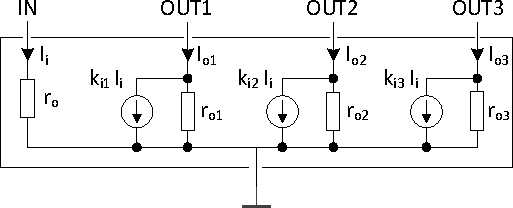
\includegraphics[width=\columnwidth, align=t]{images/06_mehrfachstromspiegel.pdf}
\end{minipage}



\subsubsection{Optimierungen für kleinstmögliche Toleranzen}

\begin{tabular}{cl}
    $V_{\rm T1} = V_{\rm T2}$               & \textrightarrow\ Beide Transistoren brauchen dieselbe konstante Temperatur    \\
    $\mu C_\text{ox1} = \mu C_\text{ox2}$   & \textrightarrow\ Matching durch gute Platzierung (Common Centroid Layout)     \\
    $\lambda_1 = \lambda_2$                 & \textrightarrow\ Identische Länge $L$ (und möglichst gross) 
\end{tabular}

\smallskip

Grundsätzlich können Stromspiegel auch in Weak- und Moderate-Inversion betrieben werden.
Dabei leidet jedoch die Genauigkeit.

% Da $V_\text{T}$ Temperaturabhängig ist, sollten die Transistoren jeweils dieselbe Temperatur haben.

% Ebenfalls ist das Teilverhältnis von $\mu C_\text{ox}$ abhängig.
% Durch kontrolliertes Platzieren der Transistoren (Common Centroid Layout) und gute Temperaturkontrolle beim Herstellen können diese Werte relativ genau gehalten werden.

% Zu guter Letzt sollten die $\lambda$ gleich gross sein.
% Dazu müssen die Transistoren dieselbe Länge $L$ (und in einem nächsten Schritt möglichst gross) sein.


\subsection{Wilson-Stromspiegel}
Der einfache Stromspiegel besitzt eine relativ tiefe Ausgangsimpedanz.
Abhilfe kann der Wilson-Stromspiegel schaffen.

$\text{N}_3$ bildet dabei eine Rückkopplung zur Regelung von $I_\text{o}$ auf $I_\text{i}$.
% TODO: How does this work? idgi...

% TODO: Schema p- und n-Wislon-Stromspiegel V7S21

% TODO: Formeln aus V7S21

\subsubsection{Verbesserter Wilson- / Kaskoden-Stromspiegel}

% TODO: Schem verbesserter Wilson- und Kaskoden-Stromspiegel V7S22

% TODO: Formeln zur minimalen Ausgangsspanung V7S23

\subsubsection{Stromspiegel mit geregelter Kaskode}

% TODO: Schema V7S24

Durch M4 und M5 wird die Spannung am Gate von M2 konstant gehalten. 
So wird die Ausgangsimpedanz bedeutend erhöht.

% TODO: Formeln V7S24

\subsection{Gegenüberstellung}

%TODO: Plots der verschidenen Varianten V7S24
% Evtl. bessere Darstellungen? Warscheindlich nicht lohnenswert.

% TODO: Tabelle aus V7S27
